% Self-contained article. Build: latexmk -pdf -interaction=nonstopmode -halt-on-error accord.tex
\documentclass[11pt,a4paper]{article}
\usepackage[T1]{fontenc}
\usepackage[utf8]{inputenc}
\usepackage{lmodern,microtype}
\usepackage[margin=25mm,headheight=15pt]{geometry}
\usepackage{amsmath,amssymb,amsthm,mathtools}
\usepackage{booktabs,tabularx,longtable,array}
\PassOptionsToPackage{nobottomtitles*}{titlesec}
\usepackage{xcolor,listings,tikz,enumitem,needspace,fancyhdr,titlesec}
\renewcommand{\bottomtitlespace}{.12\textheight}
\usepackage{xurl,etoolbox}
\usepackage[colorlinks=true,linkcolor=ink,citecolor=teal,urlcolor=teal,bookmarksnumbered=true]{hyperref}
\usepackage{bookmark}
\usetikzlibrary{arrows.meta,positioning,fit}
\definecolor{ink}{HTML}{20384D}
\definecolor{teal}{HTML}{206C75}
\definecolor{pale}{HTML}{F3F6F8}
\definecolor{muted}{HTML}{596674}
\titleformat{\section}{\Large\sffamily\bfseries\color{ink}}{\thesection}{.65em}{}
\titleformat{\subsection}{\large\sffamily\bfseries\color{ink}}{\thesubsection}{.65em}{}
\titleformat{\subsubsection}{\normalsize\sffamily\bfseries}{\thesubsubsection}{.65em}{}
\setlength{\parindent}{0pt}
\setlength{\parskip}{.42em}
\setlength{\emergencystretch}{2.5em}
\setcounter{tocdepth}{1}
\setlist{nosep,leftmargin=*}
\renewcommand{\arraystretch}{1.15}
\newcolumntype{Y}{>{\raggedright\arraybackslash}X}
\newcolumntype{P}[1]{>{\raggedright\arraybackslash}p{#1}}
\lstset{basicstyle=\small\ttfamily,columns=fullflexible,keepspaces=true,breaklines=true,
 showstringspaces=false,frame=single,rulecolor=\color{teal!35},backgroundcolor=\color{pale},
 framerule=.35pt,framesep=5pt,aboveskip=.7em,belowskip=.7em,tabsize=2}
\newcommand{\code}[1]{\nolinkurl{#1}}
\newcommand{\Accord}{\textsc{Accord}}
\newcommand{\N}{\mathbb{N}}
\newcommand{\Z}{\mathbb{Z}}
\newcommand{\Q}{\mathbb{Q}}
\newcommand{\R}{\mathbb{R}}
\newcommand{\C}{\mathbb{C}}
\newcommand{\den}[1]{[\![#1]\!]}
\newcommand{\coeff}[2]{[#1^{#2}]}
\newcommand{\guard}{\mathsf{Guard}}
\newcommand{\Spec}{\mathsf{Spec}}
\newcommand{\Checked}{\mathsf{Checked}}
\newcommand{\src}[2]{\href{#1}{#2}}
\newcommand{\design}[1]{\par\smallskip\noindent\textbf{Design decision.} #1\par\smallskip}
\newcommand{\status}[1]{\textbf{Status.} #1}
\newtheorem{proposition}{Proposition}[section]
\newtheorem{theorem}[proposition]{Theorem}
\newtheorem{lemma}[proposition]{Lemma}
\theoremstyle{definition}
\newtheorem{definition}[proposition]{Definition}
\pagestyle{fancy}
\fancyhf{}
\fancyhead[L]{\small\sffamily Accord: reasoning and certified computation}
\fancyhead[R]{\small\sffamily Second-round proposal}
\fancyfoot[C]{\small\thepage}
\hypersetup{pdftitle={Accord: A Certified Worksheet Language for Mathematical Reasoning and Symbolic Computation},pdfauthor={OpenAI, prepared for Vladimir Reshetnikov},pdfsubject={Second-round proof-language design; Lean, Leant, and verified computer algebra}}

\begin{document}
\begin{titlepage}
\color{ink}
{\sffamily\large PROOF-LANGUAGE DESIGN / SECOND ITERATION\par}
\vspace{24mm}
{\sffamily\bfseries\fontsize{39}{43}\selectfont Accord\par}
\vspace{6mm}
{\sffamily\fontsize{24}{29}\selectfont A Certified Worksheet Language\\for Mathematical Reasoning\\and Symbolic Computation\par}
\vspace{12mm}
{\large From proof obligations to a shared language\\of definitions, calculations, and arguments\par}
\vfill
\rule{\textwidth}{.8pt}
\vspace{4mm}
Prepared for Vladimir Reshetnikov\par
OpenAI\par
5 September 2026 (Pacific time)\par
\vspace{6mm}
{\small\color{muted}
A design article grounded in both Brainstorm synthesis reports and selected
ProveIt and Leant sources. The proposed language is not an implemented Lean
extension. The companion Python laboratory executes 25 narrowly scoped tests;
it is not a formally verified checker. Mathematical derivations, source
observations, proposed contracts, and executed tests are identified separately.
}
\end{titlepage}

\begin{abstract}
\noindent
The first brainstorming round converged on a sensible architecture: retain Lean
as the checking host, express mathematical steps rather than proof-state
manipulations, reconstruct scoped obligations, fix meaning before search, and
retain evidence for replay. This article accepts that architecture and proposes
a different center of gravity for the second round. \Accord{} is a
\emph{certified mathematical worksheet}: definitions, representations, exact
computations, and proof steps inhabit one typed workspace. Its computer algebra
subsystem does not merely return expressions. It returns an expression together
with a precisely classified mathematical claim: an equality, a conditional
identity, an enclosure, a specified witness, or a complete description of a
solution set. These claims cannot be silently interchanged.

The main design contribution is an observation-aware computation interface.
An algorithm may use an efficient representation without replacing the author's
mathematical object, but the interface states exactly which observations its
result preserves. This makes finite jets, coefficient calculations, algebraic
numbers, and finite reindexing available without confusing truncated data with
infinite objects, algebraic equations with root branches, or transported
identities with reflected equalities. Guarded transformations compose through
explicit evidence rather than an accumulating set of unproved assumptions.
Verified algorithms and independently checked certificates share one acceptance
boundary, with the execution path kept distinct from the correctness theorem.

Worked developments treat binomial inversion, autonomous higher derivatives,
Abel generating functions, and radical denesting. The proposal also specifies
Leant integration, a small language core, failure diagnostics, publication
artifacts, collaboration policies, an adversarial suite, and a staged evaluation
against ordinary Lean supplied with the same mathematical infrastructure.
There is no claim of measured productivity improvement, an implemented compiler,
or historical novelty for proof reflection, refinement, or declarative proof.
\end{abstract}
\clearpage
\tableofcontents
\clearpage

\section{The proposal in one page}
\label{sec:summary}
A mathematician alternates between several activities: defining an object,
choosing a useful representation, calculating, discovering a pattern, and
explaining why the pattern is true. A proof assistant and a computer algebra
system often make these feel like different workflows. \Accord{} should make
them different \emph{operations in the same mathematical document}, with the
same rules for scope, meaning, and evidence.

The fundamental unit is a \emph{mathematical transaction}. A transaction starts
from identified objects and facts, names an operation or states a claim, and
commits a result only with its exact contract. For example:
\par\noindent\begin{minipage}{\linewidth}
\begin{lstlisting}
calculate e' from e by factor over Rational
  ensuring polynomial_value(e') = polynomial_value(e)

obtain r satisfying 0 <= r and r*r = a
  by principal_real_root

claim derivative_identity on U
  by differentiate local_identity on U
\end{lstlisting}
\end{minipage}\par
These are proposed surface forms, not executable Lean syntax. The distinction
between the operations matters more than the keywords. Factoring with an equality
certificate is not a claim of irreducibility. Producing one root is not solving
an equation completely. Differentiating an identity requires an appropriate
local identity, not equality at a single point.

The design has three coupled layers. The \emph{mathematical layer} holds the
author's objects, explicit choices, and argument. The \emph{computational layer}
holds certified representations and domain algorithms. The \emph{evidence layer}
holds Lean terms, certificate checks, premises, and origins. None has permission
to silently rewrite the meaning of another.

Five decisions distinguish this proposal from another spelling of the first
round's common proof language:
\begin{enumerate}[itemsep=.25em]
\item Make the \emph{kind of a computational answer} part of its type and display.
\item Preserve mathematical objects through \emph{observation-specific representation
contracts}, rather than demand a universal canonical form.
\item Treat unproved conditions as \emph{residual obligations or conditional results},
never as newly assumed facts.
\item Give definitions and computation interfaces the same attention as proof blocks.
\item Make a small end-to-end certificate path, with invalid neighboring cases,
the first deliverable; postpone a large new grammar.
\end{enumerate}

The initial implementation should be a Lean package and editor view, not a new
kernel and not a general-purpose CAS built from scratch. Existing Lean proofs
remain first-class inputs. Leant contributes structural reconstruction and
candidate suggestions through a typed, origin-preserving service boundary.

\clearpage
\section{What the two reports establish---and what they do not}
\label{sec:reading}
\subsection{Reading scope and source identity}
Both named Brainstorm reports were read closely, including their revised
cross-comparisons, limitations, and questions for the next iteration
\cite{syn-a,syn-b}. The reading covers the common architecture, all nine proposal
profiles, the corpus audit, the Leant discussion, definition authoring, method
annotations, replay, and the proposed experiments. This article does not present
itself as a fresh full rereading or rescoring of all nine original proposals.
Their ideas are attributed through the two syntheses unless directly checked
against repository source.

The Brainstorm branch reported revision \code{494be9d5}; ProveIt's public main
reported \code{24ce8bd7}; Leant's public main reported \code{3a40904b}. Full
identities and inspected-file blob hashes appear in Appendix~\ref{app:sources}.
The syntheses also discuss newer or modified local working trees. In particular,
their ProveIt audit uses \code{7c4e3f10}, and parts of their Leant review include
uncommitted changes. Those are not silently substituted for the public source
inspected here. No ProveIt or Leant build or regression suite was run for this
article.

\subsection{The inherited core}
The six commitments emphasized in \emph{Mathematical Ideas, Checked Evidence}
are the right starting point: a Lean host, visible mathematical claims,
scoped obligations, fixed meaning, retained evidence, and fair comparisons.
The finer matrix in \emph{Nine Blueprints} makes useful distinctions within
that core. It does not establish a rival foundational architecture
\cite{syn-a,syn-b}.

The first round has already supplied good vocabulary for witness scope,
method-constrained versus checkpoint proofs, semantic edits, source-assertion
coverage, and failure outcomes. Rebranding these would not be a substantial
second-round contribution. \Accord{} adopts them and asks a more specific
question: \emph{what does this architecture become when a symbolic calculation
is a first-class mathematical action rather than a tactic that closes a hole?}

Several original emphases remain important. Loom's local contexts motivate
scoped analytical work; MPL's separation of proof and data synthesis motivates
explicit result kinds; Contour's directed views motivate representation contracts;
Mosaic's multiple proof views motivate the interface; Motive's provenance caution
limits claims about explanation; Spine's distinction between a unit and a
nonzero element protects algebraic generality. These attributions follow the
syntheses, not claims of exclusive ownership of the ideas \cite{syn-a,syn-b}.

\subsection{Three conclusions to qualify}
\textbf{An accounting layer is necessary, but may not be sufficient.}
Annotating ordinary theorems and persisting existing elaboration information is
a good first implementation strategy. It does not by itself provide a useful
interface for a symbolic result whose representation, branch, precision, or
completeness must be stated. A CAS answer can change the mathematical object
being discussed without changing any tactic keyword.

\textbf{A lexical audit measures source shape, not removable work.}
The second synthesis reports 90,637 classified entries in 1,004 FabiusFunction
files, with 32.3\% in its designated reconstruction families. Its later caveats,
and the first synthesis's critique, are essential: these percentages are not
measured author-time savings, semantic assertion coverage, or proof of successful
compilation. Here they motivate examples and instrumentation, not a performance
prediction \cite{syn-a,syn-b}.

\textbf{A provider's completeness flag is not itself an adequacy proof.}
A carefully computed losslessness flag is valuable engineering metadata.
Nevertheless, a claim about the absence of terms in a search fragment is not
a Lean proof of the original proposition's negation. A transport theorem and
its premises, or direct checked negative evidence at the original statement,
are required for that stronger conclusion. This sharpens the operational reading
of Leant's safety information in the second synthesis.

\subsection{The concrete Lean sample}
Three inspected files give different design constraints \cite{p-binomial,p-ode,p-abel}.
\begin{center}
\begin{tabularx}{\textwidth}{@{}P{.28\textwidth}YY@{}}
\toprule
Source & Work to make less intrusive & Meaning that must survive \\
\midrule
\code{BinomialInversion} & Interval/range conversion, casts, summand algebra & Integer kernels acting on any additive commutative group \\
\code{AutonomousIteratedDeriv} & Neighborhood equality and chain-rule assembly & Derivative hypotheses only at the range values actually used \\
\code{AbelPolynomialSeries} & Formal substitution, coefficient extraction, rational scalar transport & Any solution of the functional equation, over a commutative rational algebra \\
\bottomrule
\end{tabularx}
\end{center}
The public binomial-inversion corollaries and the autonomous-derivative theorem
are already reasonably compact. The objective is not to make their every line
look like prose. It is to give repeated representation work a reusable interface
without discarding the mathematical choices that make the current results good.

\section{A worksheet of objects, observations, and arguments}
\label{sec:workspace}
\subsection{Objects are not merely expression strings}
A worksheet binds an object to a resolved Lean type and term, its parameter
context, and a stable identity. The same mathematical object may have several
presentations: an expanded polynomial, a factorization, a coefficient function,
a finite array, or a graph. Presentations do not replace the object merely
because one is easier for a solver.

For example, a formal series is not an infinite printed sum to be manipulated
as text. It is an object with coefficient observations, arithmetic, and specified
substitution operations. A finite coefficient vector is a representation of
\emph{some observations} of that object, not automatically a representation of
the entire series. This distinction will do real work in the Abel example.

A fact is a proposition with evidence in a declared context. A calculation is
a request for a result and a relation to its inputs. A proof step consumes facts
and produces another fact through a checked construction. An exploratory
conjecture is visibly different from all three: it is not inserted into the fact
context, even when numerical tests are persuasive.

\subsection{The shared intermediate structure}
One typed intermediate representation should support both an ordinary Lean
frontend and a mathematical worksheet frontend. Its nodes fall into a small
number of roles:
\par\noindent\begin{minipage}{\linewidth}
\begin{lstlisting}
Object       : resolved term, type, stable identity
Assertion    : proposition, local telescope, evidence obligation
Calculation  : inputs, operation, requested result contract
Scope        : binders, assumptions, branch or neighborhood
Plan         : typed combiner, child obligations, declared method
Presentation : rendering of an identified object or assertion
\end{lstlisting}
\end{minipage}\par
The list is a specification of roles, not a claim that six record types suffice
to implement Lean elaboration. Shared metavariables and dependent substitutions
still belong to the host elaborator. The records keep the mathematical and
publication boundaries explicit.

\begin{center}
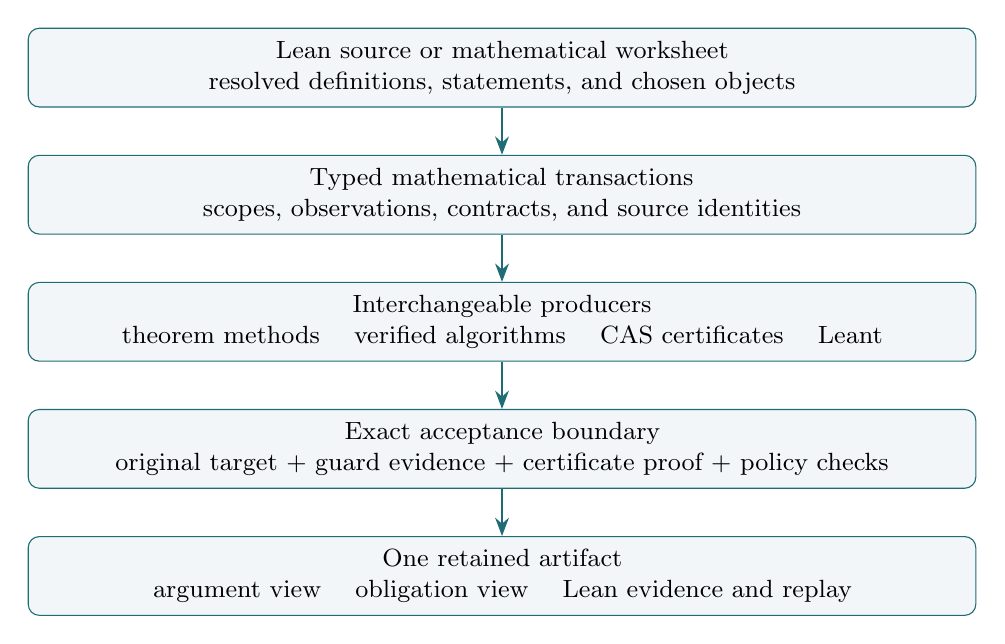
\begin{tikzpicture}[node distance=6mm,>=Stealth,
 box/.style={draw=teal,rounded corners,fill=pale,align=center,font=\small,
 text width=11.8cm,minimum height=10mm}]
\node[box] (source) {Lean source or mathematical worksheet\\resolved definitions, statements, and chosen objects};
\node[box,below=of source] (ir) {Typed mathematical transactions\\scopes, observations, contracts, and source identities};
\node[box,below=of ir] (providers) {Interchangeable producers\\theorem methods \quad verified algorithms \quad CAS certificates \quad Leant};
\node[box,below=of providers] (accept) {Exact acceptance boundary\\original target + guard evidence + certificate proof + policy checks};
\node[box,below=of accept] (archive) {One retained artifact\\argument view \quad obligation view \quad Lean evidence and replay};
\foreach \a/\b in {source/ir,ir/providers,providers/accept,accept/archive}
  \draw[->,thick,teal] (\a)--(\b);
\end{tikzpicture}
\end{center}

\subsection{Human reasoning without mind-reading}
The language should preserve a communicable argument, not claim to recover a
mathematician's private mental process. ``Introduce the inverse kernel'',
``work near this point'', and ``compare coefficients'' are decisions readers
can examine. The exact order of an author's guesses is usually not part of a
published proof.

A useful default is therefore \emph{choice-visible, consequence-collapsed}.
Show the selected map, the induction invariant, the branch, the representation,
and substantial analytic hypotheses. Collapse routine evidence for consequences
already forced by the local context. A reader can expand any step to see the
exact premises. The system must not equate ``solver closed it quickly'' with
``mathematically unimportant''.

\design{A short source is good only when its visible choices still explain the
argument and its hidden work remains available as checked evidence.}

\section{The surface language: a small core with mathematical interfaces}
\label{sec:surface}
\subsection{Keep formulas close to Lean initially}
The initial frontend should reuse Lean expressions, binders, and elaboration.
Controlled notation for sums, coefficients, and local contexts can be added as
small scoped extensions. Free-form prose may suggest an editable transaction,
but it is not authoritative input to the checker. A stored document has a
resolved, inspectable interpretation independent of whether proof search succeeds.

The core needs ordinary assertions, constructions, reductions, cases, induction,
calculations, and a Lean escape. It does not need a keyword for every mathematical
lemma. The following sketch deliberately retains familiar forms:
\par\noindent\begin{minipage}{\linewidth}
\begin{lstlisting}
theorem target (parameters) (hypotheses) : conclusion := worksheet
  let object := expression
  claim landmark : proposition by method using facts
  suffice auxiliary : proposition by bridge
  cases decidable_condition
  induct n generalizing parameters
  calculate output from input by operation
  conclude conclusion from landmark
  lean { ... }
\end{lstlisting}
\end{minipage}\par
Every listing describing \Accord{} is design pseudocode. In particular, natural
phrases such as \code{on U} or \code{from input} stand for registered typed
interfaces, not a promise that a general English parser can resolve them.

\subsection{Four operations that must not share an ambiguous meaning}
\code{claim P} creates an obligation for a proposition. \code{obtain x with P(x)
from h} eliminates an existence statement in a legal scope. \code{define x := t}
introduces a particular term. \code{select x satisfying P(x) by construction}
asks for a data-producing construction with a specification, whose accepted
choice remains stable.

The last operation cannot be implemented by unrestricted elimination from an
existence proof into computational data. The compiler must select the appropriate
host construction: a supplied dependent pair, a computable algorithm, or explicit
noncomputable choice allowed by policy. The exact choice and its specification
become part of the worksheet's object record. Lean's distinction between
propositions and computational data is substantive here \cite{lean-prop}.

A fifth operation, \code{solve all}, asks for completeness and has a stronger
contract than \code{select}. The interface should make that additional burden
visible rather than hide it in documentation for an overloaded solver command.

\subsection{Three meanings of a reason}
\code{by method M} is method-constrained: the accepted step uses the declared
contract for $M$. \code{prefer M} is search guidance: another checked proof may
be proposed, with its actual reason displayed. \code{by search} is an explicitly
open request to find evidence of the fixed claim.

\code{using only} restricts local premises, closed under dependencies needed to
type them. A separate clause controls permitted library declarations; the axiom
policy is a third control. These restrictions must not be conflated. Nor does
syntactically mentioning a permitted lemma establish that it was essential to
the proof. The method record certifies the instantiated construction, not
psychological or semantic indispensability.

\subsection{Lexical scope and stable references}
Bounded binders install their bounds as local facts. A neighborhood block installs
only the facts justified on that neighborhood. A case block owns its assumptions.
An accepted reference to ``this identity'' stores an assertion identity, not an
instruction to find whatever identity happens to precede it after editing.

An insertion that makes a displayed reference misleading should cause a rendering
change or a review notice. Deleting a referenced node creates a broken dependency,
not a request for a solver to invent a new referent. Explicit source labels remain
available when that is clearer than natural-language reference.

\section{Definitions and representation contracts}
\label{sec:representations}
\subsection{An object interface, not a new foundational object}
A definition package contains an ordinary Lean definition, selected observations,
proved interface lemmas, explicit conventions, and a scoped normalization policy.
The package does not add axioms. It makes the commitments that later proofs would
otherwise rediscover available once at the definition boundary.

For a bounded function, the author should be able to choose either a function
with a separate boundedness theorem or a bundled subtype, while the package
exposes a stable evaluation interface. For a finite sum, it can fix inclusive
endpoints and prove its bridge to \code{Finset.range}. For a formal series, it
can expose coefficient operations and their algebraic laws. These are generated
\emph{proof obligations}, not free theorems inferred from a convenient surface.

\subsection{Representation by a relation}
Let $A$ be the mathematical object type and $R$ an implementation type.
A representation contract uses a relation
\[
 V:A\to R\to\mathrm{Prop}.
\]
It may be functional, many-to-one, or partial. A decoding function and equality
$\operatorname{decode}(r)=a$ are an important special case, but not the only one.
The contract specifies which observations can cross this relation.

For an observation $o:A\to B$ and a computational observation
$\widehat o:R\to \widehat B$, a typical law is
\begin{equation}
 V(a,r)\ \longrightarrow\
 W\bigl(o(a),\widehat o(r)\bigr),
 \label{eq:observation}
\end{equation}
where $W$ is the result's own representation relation. This law is an ordinary
Lean theorem. If the operation is only valid under a guard, that premise appears
in the theorem and therefore in the obligation ledger.

The practical benefit is that an efficient representation need not support every
possible observation of its mathematical source. A truncated series can answer
low-degree coefficient questions. A numerical enclosure can answer a strict
inequality separated from zero. Neither needs, or deserves, unrestricted equality
elimination for the whole object.

\subsection{A concrete definition package: finite jets}
For a commutative ring $A$ and $N\in\N$, define the finite jet of a formal series
$F\in A[[X]]$ as its coefficients of degrees $0,\ldots,N-1$. An implementation
can use a length-$N$ array. Define
\[
 V_N(F,r)\quad\Longleftrightarrow\quad
 \forall k<N,\ r_k=[X^k]F.
\]
For $N=0$, this relation carries no coefficient information; this is legitimate,
not a corner case to infer away.

Addition acts componentwise and multiplication is truncated convolution:
\[
 (r\star s)_k=\sum_{i=0}^{k}r_i s_{k-i}\qquad(k<N).
\]
The coefficient law for series multiplication proves the representation law.
All referenced indices are below $N$, so no unseen coefficients are needed.
A compiler can discharge a concrete low-degree identity by finite computation
and transfer it through $V_N$.

It cannot conclude $F=G$ from $V_N(F,r)$ and $V_N(G,r)$. Indeed, $0$ and $X^N$
have the same first $N$ coefficients but are distinct over a nontrivial ring.
Nor does finite jet agreement imply convergence of an analytic expansion.
For a theorem quantified over all degrees, one needs a uniform coefficient
argument or a theorem quantifying over all truncation levels, not a large fixed
calculation.

Formal composition requires additional care. A safe initial jet-composition
interface requires zero constant coefficient of the inner series. More general
nilpotent-constant substitution may be supported by another proved interface;
it must not be claimed from the simpler contract. The type of observation, its
valid index range, and substitution admissibility are all part of the request.

\subsection{Transport direction and algebraic generality}
An equality proved over $\Z$ transports along a ring homomorphism to any target
ring. This does not require the homomorphism to be injective. Conversely, equality
of images generally does not imply equality of preimages. \Accord{} must record
which direction its operation needs.

Likewise, mapping a rational scalar into a commutative $\Q$-algebra does not
turn the target into a field. A nonzero rational has an inverse before mapping;
the inverse identities survive the homomorphism, even without assuming that the
target algebra is nontrivial. This is precisely the useful interface in the
Abel example. A generic ``work in a field'' transport would change its theorem.

For module-valued sums, an integer linear-combination representation is enough.
An algorithm need not multiply two module elements merely to simplify their
integer coefficients. Domain capabilities should therefore distinguish
commutative semirings, rings, modules, fields, and ordered fields instead of
routing every algebraic goal through the strongest convenient structure.

\subsection{Three-view composition and coherence}
Suppose a computation uses $V(a,r)$, then $W(r,s)$, then $Z(s,t)$. A route record
retains all intermediate representations and guards in dependency order. The
composite relation is existential relational composition, not automatic equality
of $a$ and $t$.

When two routes return different representations, the system asks what the
consumer observes. If both routes certify the same exact scalar value, a
uniqueness theorem can reconcile them. If they choose roots, bases, orderings,
or normal forms, their outputs may not be interchangeable. Either a proved
coherence law for the required observation or an explicit author choice is needed.
A path search that simply selects the first successful route is not an acceptable
meaning-resolution policy.

\design{Automate a representation change only within a declared observation
contract. Changing a branch or an accepted data object remains a reviewable edit.}

\section{The type of a computational answer}
\label{sec:answers}
\subsection{Results are not interchangeable assurances}
A symbolic operation should have an input type, an output type, and an exact
specification. The following distinctions are small enough for a first
implementation and strong enough to prevent many misleading CAS interactions.
\begin{center}
\begin{tabularx}{\textwidth}{@{}P{.22\textwidth}YP{.28\textwidth}@{}}
\toprule
Result kind & Mathematical content & What it does not establish \\
\midrule
Identity & $\den e=\den {e'}$ in a stated context & A preferred or unique normal form \\
Conditional identity & $G\to\den e=\den {e'}$ & That $G$ holds \\
Enclosure & $a\leq x\leq b$, with exact endpoints & $x$ equals a displayed decimal \\
Witness & $w:A$ together with $P(w)$ & Uniqueness or all solutions \\
Complete solution description & $\forall x,\ P(x)\leftrightarrow x\in S$ & An ordering or canonical representative unless specified \\
Observation agreement & $o(a)=\widehat o(r)$, or a stated relation & Interchangeability under arbitrary observations \\
Counterexample & A specified input violating the original universal claim & That a different, stronger claim is false \\
\bottomrule
\end{tabularx}
\end{center}

These are not merely colored user-interface badges. A consumer requesting an
identity cannot accept an enclosure. A consumer requiring all solutions cannot
accept a list of independently verified witnesses. Conversion between kinds is
an ordinary mathematical operation with its own theorem. An enclosure $a\le x$
with $a>0$ gives $x>0$; it does not give an exact expression for $x$.

It is useful to separate an answer's \emph{mathematical kind} from its
\emph{validation state}. ``Witness'' is a kind. ``Proposed'', ``checked in this
session'', and ``independently replayed'' are states. ``Conditional'' describes
remaining mathematical premises, not a weakened notion of correctness. A fully
checked theorem $G\to P$ is rigorous even when $G$ has not been proved.

\subsection{A dependent interface}
The logical interface can be expressed schematically in Lean-like notation:
\par\noindent\begin{minipage}{\linewidth}
\begin{lstlisting}
structure Operation where
  Input  : Type
  Output : Input -> Type
  Spec   : (i : Input) -> Output i -> Prop

structure CertifiedAnswer (op : Operation) (i : op.Input) where
  value    : op.Output i
  evidence : op.Spec i value
\end{lstlisting}
\end{minipage}\par
This is a conceptual interface, omitting universes, local telescopes, serialization,
and host-specific details. In a real implementation, the evidence field must be
constructed or imported through the exact checking boundary. An external JSON
record containing a field named \code{evidence} is not such a dependent pair.

The request fixes \code{op}, the elaborated input, the expected specification,
and the relevant context. A provider may propose an output, but cannot redefine
\code{Spec} to fit what it happened to find. Result data shared with later
obligations is committed transactionally so that the specification refers to the
same chosen output everywhere.

\subsection{Soundness versus completeness of algebraic answers}
For a polynomial $p$, a product identity
\[
 p=c\prod_{i=1}^{m}q_i^{e_i}
\]
certifies a factorization in a weak, useful sense. Calling it an irreducible
factorization additionally requires irreducibility, suitable nonunit conditions,
and any normalization convention used to select $c$ and the $q_i$. Calling it
canonical requires a uniqueness statement relative to those conventions.

For an equation $P(x)$, checking $P(a_1),\ldots,P(a_m)$ certifies listed
solutions. Completeness requires the reverse implication that every solution
belongs to the represented set. A real-root isolator may establish that disjoint
intervals each contain one root and that there are no roots outside them. The
root-count and coverage evidence is not optional because the individual root
certificates already look convincing.

A similar distinction applies to linear algebra. A vector $x_0$ with $Ax_0=b$
is a witness. A basis for $\ker A$ together with $x_0$ gives all solutions only
when both independence and spanning have the required evidence. A certificate
of a residual equation alone is insufficient.

\subsection{Exact output and approximate presentation}
A decimal can be a display of an exact object, an exact rational literal, or an
approximation. These should render differently. A certified enclosure is stored
with rational or otherwise exact endpoints and an inequality theorem. A decimal
printer may shorten the display, but cannot change the recorded interval.

For strict inequalities, the interface should report the separation that made
the proof possible. If an enclosure contains zero, the result is inconclusive
for a sign request. Increasing precision is a new computation, not a reason to
pretend that zero was excluded. Equality of general real expressions is not
made decidable by a precision setting.

\section{Verified algorithms and certificate-producing computer algebra}
\label{sec:cas}
\subsection{Two implementation routes, one logical boundary}
A hybrid system should support both formally verified algorithms and arbitrary
candidate-generating algorithms with verified checkers. They solve different
engineering problems.

In the first route, an algorithm $f:I\to O$ has a proved correctness theorem
\[
 \forall i,\ \Spec(i,f(i)).
\]
This is valuable for small normalizers, exact arithmetic, structured array
operations, and algorithms whose implementation can be efficiently refined.
But the theorem does not authenticate an arbitrary output from an external
execution of $f$. To accept the concrete output $o$, the system also needs
checked evidence that $f(i)=o$, or another checked path from $i$ and $o$ to
$\Spec(i,o)$.

In the second route, an untrusted program proposes an output $o$ and a certificate
$c$. A formally specified checker has a soundness theorem
\begin{equation}
 \operatorname{check}(i,o,c)=\mathsf{true}
 \quad\longrightarrow\quad \Spec(i,o).
 \label{eq:checker}
\end{equation}
The checker is usually simpler than the search algorithm. An expensive
factorization, search for a polynomial identity, or heuristic simplification can
then be replaced without changing the acceptance rule.

\design{A correctness theorem for an algorithm and trustworthy evidence of a
particular execution are separate obligations. Do not use the first as a license
to trust arbitrary native output.}

Lean's current validation guidance distinguishes native computation assumptions
from ordinary kernel checking, and documents per-computation axioms from Lean
4.29 onward. A strict \Accord{} profile should instead use kernel-justified
reduction or reconstructed certificate proofs, and audit the actual transitive
axiom inventory rather than blacklist a historical constant name
\cite{lean-validation}.

\subsection{The reification boundary}
A certificate checker commonly operates on reified syntax: sparse polynomials,
rational expressions, linear combinations, or finite arrays. The original goal
contains Lean expressions. The link between them is part of the proof.

For example, a polynomial reifier may treat $\sin x$ and $\exp y$ as opaque atoms
and prove that the source expression denotes a polynomial in those atoms. The
polynomial certificate can then prove a ring identity without proving anything
about sine or exponential. It must not equate two atoms because their printed
names happen to coincide, or because a simplifier guessed an analytic identity.
Each atom is bound to an exact expression in its local context.

There are two acceptable patterns. A proved reifier produces the relation
between source syntax and its interpretation. Alternatively, an untrusted
reifier emits a proposed translation together with a Lean equality that is
independently checked. Neither pattern makes a pretty-printer part of the
mathematical authority.

\subsection{Polynomial identities under hypotheses}
Suppose the context provides $f_1(x)=0,\ldots,f_m(x)=0$. To prove $p(x)=0$, a
producer may return polynomials $q_1,\ldots,q_m$ satisfying the identity
\begin{equation}
 p=\sum_{i=1}^{m}q_i f_i.
 \label{eq:idealcertificate}
\end{equation}
A coefficient-normalization checker verifies this finite polynomial identity.
Evaluation and the context equations then prove the target. The producer may
find the $q_i$ by any method; its search algorithm need not be trusted.

This proves a sufficient certificate of ideal membership. It does not make a
failed search a proof of nonmembership, and it is not a complete procedure for
all consequences over every coefficient domain. An ordered-field inequality,
radical branch, or cancellation requires additional information. In the radical
example below, equation~\eqref{eq:idealcertificate} verifies the square, while
an order theorem selects the correct square root.

For noncommutative input, a commutative polynomial checker is the wrong
operation. The reification contract must require the actual algebraic capability
used by the normalization theorem. This check belongs before accepting a
certificate, not in an informal warning after the calculation succeeds.

\subsection{Conditional rational simplification}
A rational-expression normalizer should carry its domain information. Cross
multiplication of $a/b=c/d$ is justified by $b\ne0$ and $d\ne0$ for the usual
field argument. Polynomial equality of $ad$ and $bc$ by itself does not prove
the equality of the original totalized divisions at their poles.

A calculation may therefore return
\[
 (x\ne0)\ \longrightarrow\ x/x=1.
\]
If $x\ne0$ follows from existing context, the worksheet discharges it and
commits the equality. Otherwise it can retain the conditional identity, ask
for a case split, or propose a globally valid piecewise result. It must not
strengthen the theorem statement by quietly adding $x\ne0$.

A guard is attached to the exact operation and expression. Caching a certificate
for cancellation at one nonzero denominator cannot authorize cancellation of a
similar-looking expression in another branch. Likewise, natural subtraction
and natural division need their own transport laws; field algebra does not
supply them.

\subsection{Finite sums as symbolic certificate problems}
Many symbolic summations can be accepted through local identities plus boundary
information rather than by trusting a general summation command. Consider
\[
 F(k)=\frac1{k(k+1)},\qquad
 G(k)=\frac1k,\qquad k\ge1.
\]
The certificate $F(k)=G(k)-G(k+1)$ follows by exact field algebra under the
nonzero-denominator guards. Finite telescoping then yields, for $n\in\N$,
\[
 \sum_{k=1}^{n}\frac1{k(k+1)}=1-\frac1{n+1}=\frac n{n+1}.
\]
At $n=0$, the sum is empty and the result is zero. The proof does not evaluate
the singular expression $G(0)$, and the certificate interface must not create
that spurious boundary term.

More general recurrence certificates need an identity for the summand, valid
index ranges, boundary contributions, initial values, and a theorem that the
recurrence determines the requested sequence. A recurrence without its initial
conditions is not a closed-form proof. An identity obtained by clearing
denominators needs a separate argument at any indices where those denominators
vanish. These are natural first-class certificate fields.

\subsection{Integration, differential equations, and limits}
A symbolic antiderivative is an excellent example of an incomplete-looking
answer that can nevertheless have a precise useful contract. The operation
may return $F$ and a proof of $F'=f$ on $U$. Evaluating a definite integral then
requires the appropriate fundamental-theorem hypotheses and endpoint treatment.
An improper integral additionally needs limiting evidence. The derivative
certificate does not grant these facts.

Likewise, a proposed solution of an ordinary differential equation can carry a
proof of the equation and initial value. Uniqueness, maximality, and a claimed
domain of existence are separate specifications. A formal power-series solution
is not automatically an analytic solution. \Accord{} should expose these
modular guarantees instead of making a general \code{solve} command appear
more complete than its evidence.

\subsection{Suggested initial algorithm inventory}
\begin{longtable}{@{}P{.24\textwidth}P{.37\textwidth}P{.31\textwidth}@{}}
\toprule
Operation & Initial acceptance evidence & Explicit boundary \\
\midrule
\endhead
Exact scalar arithmetic & Kernel-justified rational/integer calculation & No floating-point equality oracle \\
Polynomial normalization & Equality to a reified polynomial normal form & Correct coefficient structure and atom identity \\
Consequence of polynomial equations & Identity~\eqref{eq:idealcertificate} and premise proofs & No negative result from failed certificate search \\
Finite reindexing & Bijection or explicit multiplicity theorem & No rearrangement of infinite sums \\
Rational simplification & Polynomial certificate plus denominator guards & Totalization and exceptional cases retained \\
Finite jets & Truncated arithmetic and observation transport & Only the certified coefficient range \\
Real algebraic roots & Defining polynomial, root isolation, count/branch evidence & Witness versus complete root set distinguished \\
Numerical bounds & Exact enclosure and error evidence & A decimal display is not the theorem \\
Differentiation & Syntax-directed rules and locality/regularity premises & Pointwise identity is insufficient for derivative transfer \\
\bottomrule
\end{longtable}
This is a capability roadmap, not a list of newly implemented Lean algorithms.
Several entries can reuse existing proof-producing tactics. New work should
concentrate on exact requests, reusable interfaces, result classification,
representation bridges, and evidence persistence before reimplementing a mature
normalizer.

\section{Guards, observations, and compositional guarantees}
\label{sec:composition}
\subsection{Conditional results are legitimate objects}
A calculation under unresolved conditions produces a theorem with those
conditions as premises. It does not create trusted assumptions. For a fixed
context $\Gamma$, a result may have the form
\[
 p:\Pi(h_1:G_1)\cdots(h_m:G_m).\ R(e,e'),
\]
where later guards may depend on earlier choices and proofs. The ledger records
which guards have evidence and which remain open. The result $R(e,e')$ can be
used unconditionally only after the required arguments have been supplied.

This permits useful exploration: a user can inspect a conditional simplification
without committing to its applicability. Publication may include the conditional
claim as such. It cannot print the unconditional equality under the same badge.

\subsection{A relational composition rule}
The following rule makes explicit what a computation pipeline must establish.
It is a mathematical specification, not a verified compiler metatheorem.

\begin{proposition}[Guarded observation composition]
Let $V\subseteq A\times R$, $W\subseteq R\times S$, and
$Z\subseteq B\times T$. Suppose the context contains $V(a,r)$. Let an
algorithm produce $s$ and evidence
\[
 G(a,r)\longrightarrow W(r,s).
\]
Suppose a consumer observation has a proved bridge
\[
 V(a,r)\land W(r,s)\land H(a,r,s)
 \longrightarrow Z\bigl(o(a),q(s)\bigr).
\]
Then the pipeline establishes
\[
 G(a,r)\land H(a,r,s)
 \longrightarrow Z\bigl(o(a),q(s)\bigr).
\]
It establishes the conclusion without those premises only when the context
also supplies evidence of both guards.
\end{proposition}
\begin{proof}
Assume the two guards. Apply the algorithm's checked implication to obtain
$W(r,s)$. Combine it with the existing $V(a,r)$ and the consumer guard; the
bridge theorem gives the desired result. No inverse to $V$ or $W$, and no
unmentioned preservation property, was used. Without guard evidence the same
construction is a function of the guards, hence only a conditional result.
\end{proof}

The rule is deliberately relational. It covers a finite jet answering one
coefficient query just as well as an exact representation answering equality.
It also explains why the order of dependent guards matters: a condition on a
chosen $s$ cannot be discharged against another candidate $s'$ and then reused
by spelling.

\subsection{No strengthening by composition}
Let the worksheet's permitted assumptions be the ordered context $\Gamma$.
Each transformation may either use a premise already derivable in $\Gamma$ or
return that premise as an explicit antecedent. A case split may introduce a
premise in a new branch, with a checked eliminator covering all cases. Under
these rules, composition cannot silently add hypotheses to a public theorem.

This is more useful as a compiler invariant than as another broad soundness
slogan. Every accepted edge has a list of \emph{used} assumptions with evidence
and a list of \emph{residual} conditions. There is no operation ``promote all
conditions returned by the CAS to assumptions''. The final theorem and every
asserted intermediate node are checked at their approved types.

\subsection{Observation strength is not a single linear scale}
An exact enclosure and a factorization may both be highly informative, but
neither is uniformly stronger than the other. A finite jet determines certain
coefficients exactly and says nothing about many other observations. Rather
than assign an undifferentiated confidence score, each consumer requests a
specific relation, and registered theorems justify conversions between relations.

A particularly important forbidden conversion is
\[
 \bigl(\forall k<N,\ [X^k]F=[X^k]G\bigr)
 \ \not\Longrightarrow\ F=G.
\]
A permitted conversion is coefficient equality for a particular $k<N$. Another
is an equality theorem for polynomials of degree strictly less than $N$, provided
those degree bounds are proved. The bounds are part of the bridge, not an
optimization hint.

\subsection{Shared constraints and transactional acceptance}
Two obligations may share an output term, a type, an instance, or a universe
constraint. Solving them as independent jobs and merging their text is unsafe.
The host worker must either close them over fixed interfaces or use a transaction
that checks all assignments for compatibility before committing.

For example, a root provider might solve an equation with one branch while a
sign provider proves a property of another. Both individual messages can be
correct in isolation. Only a shared identity for the root makes their conjunction
meaningful. The same issue arises when a coefficient domain is inferred in one
subgoal and an instance in another. The scheduler must not treat a dependency
DAG as a substitute for the dependent elaboration state.

\subsection{Conditional rewriting and equality saturation}
Maintaining several equivalent expressions can be useful: a factorization for
sign reasoning, an expansion for coefficient comparison, and a Horner form for
evaluation. An optional equality-saturation engine could explore these forms.
It must merge equivalence classes only when the required equality is established
in the exact scope. A rewrite valid under an unresolved guard is a guarded edge,
not unconditional equality.

Binder scope, branches, and representation observations therefore partition the
search space. A simplification learned under $x>0$ cannot leak to a sibling
branch where $x<0$. A small initial implementation should use directed,
versioned normalization policies and explicit transformations. Equality
saturation is a later optimization, not a required foundation or a source of
new mathematical authority.

\section{Worked example I: binomial inversion without a field}
\label{sec:binomial}
\subsection{The mathematical argument}
Let $M$ be an additive commutative group, and let $a,b:\N\to M$ satisfy
\[
 b_n=\sum_{k=0}^{n}\binom nk\,a_k,
\]
where the coefficients act by integer scalar multiplication. Define
\[
 K(n,k)=(-1)^{n-k}\binom nk\in\Z.
\]
The key scalar identity is
\begin{equation}
 \sum_{k=j}^{n}(-1)^{n-k}\binom nk\binom kj=\delta_{nj}.
 \label{eq:binomialkernel}
\end{equation}
If $n<j$, the interval is empty and both sides are zero. Otherwise write
$n=j+m$ and substitute $k=j+i$. The map
\[
 i\longmapsto j+i:\{0,\ldots,m\}\longrightarrow\{j,\ldots,n\}
\]
is a bijection. For $0\leq i\leq m$, the binomial product identity gives
\[
 \binom{j+m}{j+i}\binom{j+i}{j}
 =\binom{j+m}{j}\binom mi,
\]
and $n-k=m-i$. Thus the left side of~\eqref{eq:binomialkernel} becomes
\[
 \binom nj\sum_{i=0}^{m}(-1)^{m-i}\binom mi.
\]
The alternating binomial row is one when $m=0$ and zero otherwise. In the first
case $n=j$ and $\binom nj=1$; in the second case the product vanishes. This proves
the identity in all cases.

Substituting the formula for $b_k$ and interchanging the finite triangular sum,
\begin{align*}
 \sum_{k=0}^{n}K(n,k)\,b_k
 &=\sum_{j=0}^{n}
   \left(\sum_{k=j}^{n}K(n,k)\binom kj\right)a_j\\
 &=\sum_{j=0}^{n}\delta_{nj}a_j=a_n.
\end{align*}
Only the laws of an additive commutative group and its integer scalar action
are needed for this second step. There is no multiplication of two elements
of $M$, no division in $M$, and no embedding of $M$ into a field.

\subsection{The proposed worksheet}
\par\noindent\begin{minipage}{\linewidth}
\begin{lstlisting}
claim kernel_orthogonality (n j : Nat) : kernel_sum n j = delta n j
  cases n < j
  case empty:
    conclude by empty_interval
  case bounded:
    obtain m with n = j + m by natural_difference
    reindex kernel_sum by k := j + i, i in [0..m]
    rewrite each summand by binomial_product
    collect the constant factor
    conclude by alternating_binomial_row

claim inversion in AddCommGroup M
  substitute the definition of b
  interchange the finite triangular sum
  apply kernel_orthogonality to the coefficient of each a j
\end{lstlisting}
\end{minipage}\par
The displayed map and the kernel identity are the mathematical decisions.
The operation package generates the interval membership, injectivity, coverage,
subtraction, coefficient-cast, and scalar-distribution obligations. The author
can expand them, but should not have to spell them out on every reuse.

The actual ProveIt file already extracts a lower-triangular kernel framework,
and its public module-valued result applies that framework rather than repeating
the double sum. Its scalar proof contains the interval conversion, binomial
product, arithmetic, and cast steps described above \cite{p-binomial}. The
worksheet should reuse these library assets, not disguise the whole target
theorem as a new method called \code{binomial_magic}.

\subsection{The concrete operation contract}
For finite sets $S,T$, a map $f:S\to T$, and summands in an additive commutative
monoid, the method requires membership preservation, injectivity on $S$, coverage
of $T$, and the specified equality of corresponding summands. Equivalently, the
author can supply a bundled finite equivalence. The theorem application is the
logical contract; annotations specify which input is the chosen map and which
premises a local routine profile may try.

In this example, coverage follows because for $k\in\{j,\ldots,j+m\}$,
$i=k-j$ satisfies $0\le i\le m$ and $j+i=k$. The proof uses the bound $j\le k$;
that bound is local to the target interval. Natural subtraction is not being
reinterpreted as integer subtraction globally.

\subsection{Discriminating negative cases}
Changing the source interval to $\{0,\ldots,m-1\}$ omits the upper endpoint
when $m>0$. The named reindexing method should fail at coverage and identify
$k=n$ as the missed endpoint in a concrete counterexample. A broad solver might
prove the ultimate theorem another way, but it must not preserve the false
explanation that this map was a bijection.

A noninjective map needs a multiplicity theorem rather than the same bijection
contract. An infinite sum needs an appropriate summability or rearrangement
argument. Changing $M$ to a commutative field is a statement change even if it
makes a normalizer applicable. All three are valuable tests because an interface
that merely accepts the positive example can conceal these mistakes.

\section{Worked example II: local differentiation as a context operation}
\label{sec:derivative}
\subsection{The exact generality to preserve}
Let $U\subseteq\R$ be open. Suppose $W,\varphi:\R\to\R$, and for every $x\in U$,
$W$ has derivative $\varphi(W(x))$ at $x$. Let $G_n,H_n:\R\to\R$ satisfy
\begin{align*}
 G_0(W(x))&=W(x),\\
 G_n'\bigl(W(x)\bigr)&=H_n(W(x)),\\
 G_{n+1}(W(x))&=H_n(W(x))\varphi(W(x))
 \qquad (x\in U).
\end{align*}
The middle line means an actual derivative-existence assertion at the indicated
point, not merely an equality involving a total derivative operator. Nothing
requires $G_n$ to be differentiable everywhere.

Then
\begin{equation}
 W^{(n)}(x)=G_n(W(x))\qquad(n\in\N,\ x\in U).
 \label{eq:ode}
\end{equation}
These are the essential hypotheses of ProveIt's
\code{AutonomousODE.iteratedDeriv_eq_comp}, whose source explicitly keeps the
assumptions local to the range of $W$ over $U$ \cite{p-ode}.

\subsection{Why the induction hypothesis must remain local}
The case $n=0$ follows from the first hypothesis. Assume the identity for every
point of $U$, and fix $x\in U$. Openness makes $U$ a neighborhood of $x$, so
$W^{(n)}$ and $G_n\circ W$ agree near $x$. Derivative congruence and the chain
rule give
\[
 W^{(n+1)}(x)
 =H_n(W(x))W'(x)
 =H_n(W(x))\varphi(W(x))
 =G_{n+1}(W(x)).
\]
The neighborhood equality is not extraneous proof bureaucracy. It is the reason
that differentiating the induction identity is valid. The formal plumbing that
constructs this equality can be conventional and reusable, while the locality
itself remains visible in the argument.

\par\noindent\begin{minipage}{\linewidth}
\begin{lstlisting}
induct n with invariant:
  for every x in U, D[n] W x = G[n] (W x)
case zero:
  conclude from initial_identity
case successor:
  fix x in U
  work near x inside U using openness
  differentiate the induction identity
  use the chain rule, the equation for W, and the recurrence for G
\end{lstlisting}
\end{minipage}\par

\subsection{A theorem-backed local interface}
The basic transfer interface takes eventual equality near $x$ and a derivative
proof for one function, and returns a derivative proof for the other. A separate
adapter turns equality on an open set containing $x$ into eventual equality.
The composite can be registered as one mathematical operation, but its underlying
lemmas remain ordinary Lean library assets.

A locality record should contain the filter or neighborhood, its membership
proofs, and exactly the facts valid there. Restriction to a smaller neighborhood
is a theorem-backed operation. Merely using the phrase ``near $x$'' does not
synthesize arbitrary regularity assumptions.

This also suggests an economical CAS role. A syntax-directed derivative engine
can compute the derivative expression for $G_n\circ W$, but its result is a
conditional \code{HasDerivAt} theorem. The surrounding proof layer supplies the
local derivative hypotheses and the equation for $W$. Neither subsystem has to
pretend to solve the entire analysis problem alone.

\subsection{The negative neighbor and the honest diagnostic}
The functions $f(t)=0$ and $g(t)=t$ satisfy $f(0)=g(0)$ but have different
derivatives at zero. Replacing the induction identity on $U$ by equality only
at the chosen point therefore destroys the local-transfer step.

A useful diagnostic is: ``This differentiation uses equality on a neighborhood
of $x$; the available fact is equality at $x$ only.'' It should highlight the
missing proposition and the supplying induction invariant. It should not add
openness or global differentiability to the public statement without review.
An explicitly proposed stronger induction invariant is a plan edit, not a silent
routine inference.

\section{Worked example III: Abel coefficients over a rational algebra}
\label{sec:abel}
\subsection{Formal series and arbitrary solutions}
Let $A$ be a commutative $\Q$-algebra and $a,x\in A$. Work with formal power
series, not analytic functions. Suppose an arbitrary series $T$ satisfies
\[
 T=t\exp(-aT).
\]
Its constant coefficient is zero, so the required formal substitutions are
admissible under the zero-constant-term interface. The goal is the coefficient
identity
\begin{equation}
 [t^{n+1}]\exp(xT)
 =\iota\!\left(\frac1{(n+1)!}\right)
       x\bigl(x-(n+1)a\bigr)^n,
 \label{eq:abel}
\end{equation}
where $\iota:\Q\to A$ is the algebra map and natural scalars in $A$ are understood
through their canonical action.

The actual ProveIt theorem applies to any $T$ satisfying the functional equation.
The source separately provides a canonical construction \code{abelSeries}; it
does not substitute that construction for an arbitrary solution in the
coefficient theorem \cite{p-abel}. Preserving this distinction is a direct test
of the proposed language's object discipline.

\subsection{The coefficient calculation}
Write $m=n+1>0$. The appropriate formal Lagrange--B\"urmann theorem gives
\[
 [t^m]\exp(xT)
 =\iota(1/m)\,[u^{m-1}]
   \left(x\exp(xu)\exp(-mau)\right).
\]
Combining exponentials and extracting the known coefficient yields
\begin{align*}
 [t^m]\exp(xT)
 &=\iota(1/m)\,x\,[u^{m-1}]\exp((x-ma)u)\\
 &=\iota(1/m)\,x\,(x-ma)^{m-1}\iota(1/(m-1)!)\\
 &=\iota(1/m!)\,x\,(x-ma)^{m-1}.
\end{align*}
The last step is rational scalar arithmetic transported through $\iota$.
Equation~\eqref{eq:abel} follows by $m=n+1$. Degree zero is treated separately:
$\exp(xT)$ has constant coefficient one.

No field inverse of an arbitrary element of $A$ has been used. The scalar
cancellation needed in a derivative-based version of the Lagrange theorem is
\[
 \iota(1/m)\,\iota(m)=\iota((1/m)m)=1.
\]
It is proved in $\Q$ using $m>0$, then transported. There is no need to assume
that $A$ is a field or that $\iota$ is injective. This matches the source's
explicit cancellation and factorial steps \cite{p-abel}.

\subsection{A coefficient compiler, not a universal series solver}
\par\noindent\begin{minipage}{\linewidth}
\begin{lstlisting}
context formal_series over commutative Rational_algebra A
  given T satisfying T = t * exp(-a*T)
  derive constant_coefficient(T) = 0

claim coefficient_formula (n : Nat)
  apply formal_Lagrange_Burmann at degree n+1
  combine formal exponentials
  extract the exponential coefficient
  normalize Rational scalars through algebraMap

claim full_series_identity
  compare coefficients
  handle degree zero separately
  use coefficient_formula at positive degrees
\end{lstlisting}
\end{minipage}\par
The compiler's trusted mathematical ingredients are the specific Lagrange theorem,
formal exponential laws, coefficient laws, and scalar-transport theorems.
Its search or reification strategy is not mathematical evidence. The author has
selected the generating-function argument and the coefficient observation;
these choices are not hidden behind a generic solver invocation.

Concrete coefficients can use finite jets and verified truncated multiplication.
The quantified formula needs the symbolic coefficient theorem above. This is a
useful division of labor: the same definition package supports exact experiments
and general proofs while preserving the difference between them.

\subsection{The binomial-type identity as an observation}
Define $A_0(a,x)=1$ and
$A_m(a,x)=x(x-ma)^{m-1}$ for $m\ge1$. The coefficient formula gives the formal
exponential generating function
\[
 \exp(xT)=\sum_{m\ge0}\iota(1/m!)A_m(a,x)t^m.
\]
Since $\exp((x+y)T)=\exp(xT)\exp(yT)$, coefficient comparison and rational
factorial arithmetic give
\[
 A_n(a,x+y)=\sum_{k=0}^{n}\binom nk
                     A_k(a,x)A_{n-k}(a,y).
\]
The product formula is an ordinary formal-series theorem. The compiler can
render the high-level coefficient argument while retaining the finite convolution
and scalar proofs underneath. This is where the CAS and proof language genuinely
cooperate: computation supplies the coefficient normal forms, while the proof
supplies the reason they belong to the same formal identity.

\subsection{Three failures worth testing}
A finite jet calculation at degree 50 does not establish the theorem for all
$n$. An analytic rendering of the same series does not establish convergence
or permission to evaluate it at a real number. Replacing arbitrary $T$ by the
canonical \code{abelSeries} narrows a quantified claim unless a separately
stated argument justifies the substitution. Each invalid move can produce a
plausible-looking page; the typed contracts are what make the errors visible.

\section{Worked example IV: branch-safe radical denesting}
\label{sec:radicals}
\subsection{The smallest complete certificate}
Consider the real principal square root identity
\begin{equation}
 \sqrt{3+2\sqrt2}=1+\sqrt2.
 \label{eq:radicalsmall}
\end{equation}
Let $r=\sqrt2$ and $q=1+r$. The defining properties give $r\ge0$ and $r^2=2$.
Then $q\ge0$, and the polynomial certificate
\[
 (1+r)^2-(3+2r)=r^2-2
\]
proves $q^2=3+2r$. Since a nonnegative real number with this square is the
principal root, equation~\eqref{eq:radicalsmall} follows.

The certificate separates two tasks. Polynomial algebra proves the square.
Order and root uniqueness prove the branch. The candidate $-1-r$ has exactly
the same square and must be rejected by a principal-root request. A system that
only checks a minimal polynomial or a squared identity will miss this distinction.

\par\noindent\begin{minipage}{\linewidth}
\begin{lstlisting}
calculate sqrt(3 + 2*sqrt(2)) by denest over Real
  let r := principal_root(2)
  propose 1 + r
  certify its square by polynomial_combination
  certify its nonnegativity by ordered_algebra
  conclude by uniqueness_of_nonnegative_square_root
\end{lstlisting}
\end{minipage}\par
The producer may be an external CAS or a specialized search engine. The accepted
value is attached to the same branch specification as the original request.
The proof package remains valid even when another producer proposes the same
answer by a different search strategy.

\subsection{A reusable rational denesting certificate}
The previous example is an instance of a more useful theorem. It specifies
what a restricted denesting algorithm can certify without claiming to solve
every radical-denesting problem.

\begin{theorem}[A two-square-root certificate]
Let $a,b,c,d\in\Q$, interpreted in $\R$, satisfy
\[
 a\ge0,\qquad c\ge0,\qquad d\ge0,\qquad d^2=a^2-b^2c.
\]
Put $u=(a+d)/2$ and $v=(a-d)/2$. Then $u\ge v\ge0$ and
\[
 \sqrt{a+b\sqrt c}
 =\begin{cases}
   \sqrt u+\sqrt v,& b\ge0,\\
   \sqrt u-\sqrt v,& b<0.
  \end{cases}
\]
All square roots are nonnegative real square roots.
\end{theorem}
\begin{proof}
Since $a^2-d^2=b^2c\ge0$ and $a,d\ge0$, we have $a\ge d$.
Consequently $u\ge v\ge0$. Direct calculation gives
\[
 u+v=a,\qquad uv=\frac{b^2c}{4}.
\]
Both $2\sqrt u\sqrt v$ and $|b|\sqrt c$ are nonnegative, and their squares
are $4uv=b^2c$. Uniqueness of the nonnegative square root therefore gives
$2\sqrt u\sqrt v=|b|\sqrt c$.

For $b\ge0$, the square of $\sqrt u+\sqrt v$ is
$a+|b|\sqrt c=a+b\sqrt c$, and the sum is nonnegative.
For $b<0$, the square of $\sqrt u-\sqrt v$ is
$a-|b|\sqrt c=a+b\sqrt c$. Moreover $u\ge v$ implies
$\sqrt u\ge\sqrt v$, so the difference is nonnegative as well.
In each case its square is the requested radicand, which in particular proves
that radicand is nonnegative. Root uniqueness finishes the argument.
\end{proof}

The theorem also holds for real parameters satisfying these premises, but the
rational version explains the computational benefit: an exact rational $d$
makes $u$ and $v$ rational, leaving only unnested square roots. The producer may
try to find $d$ by an exact rational square-root calculation; the checker need
only establish its sign and square identity. Failure to find such a $d$ means
this particular certificate was not obtained, not that the original expression
has no denesting in a broader language.

Examples are $(a,b,c,d)=(3,2,2,1)$, giving $\sqrt2+1$, and
$(3,-2,2,1)$, giving $\sqrt2-1$. The latter is a good branch test: reversing the
order of the two roots preserves the square but violates nonnegativity.
The case $b=0$ is covered without division by $b$; degeneracies are part of the
theorem rather than numerical exceptions in the algorithm.

\subsection{Algebraic number representations}
A larger algebraic-number package should identify a real number by a defining
polynomial and enough isolating information to select the intended root. Two
numbers satisfying the same polynomial need not be equal. An equality checker
must establish that the represented roots coincide, not merely compare their
polynomials. Polynomial irreducibility or a minimal-polynomial convention may
improve representation, but does not replace branch information.

This direction has concrete verified precedents outside Lean: the Archive of
Formal Proofs contains algebraic-number arithmetic and root computations, as
well as verified Sturm-sequence constructions and root-count methods
\cite{afp-algebraic,afp-sturm}. They support feasibility of the mathematical
components, not a claim that the required Lean package is already available.

\subsection{Certificates for exactness, not just a prettier expression}
The denesting result has a precise relation to the input. A separate presentation
policy may prefer fewer nested roots or shorter printed terms. Proving that an
expression is globally shortest among all radical expressions is a much stronger
optimization claim and is not part of this operation.

The same separation handles $\sqrt{x^2}=|x|$. Replacing the right side by $x$
requires a sign condition; in the absence of that condition, the absolute-value
form is the exact unconditional answer. The system should not treat it as an
inferior failure to simplify.

\section{Leant as a provider, not a second authority}
\label{sec:leant}
\subsection{Preserve its useful distinctions}
Leant already separates structural term generation from Lean acceptance. Its
README describes a REPL that synthesizes terms, checks candidates through the
Lean backend, and offers interactive proving. The inspected fragment module
records the structural translation and conservatively marks unsupported or
potentially unsafe content for negative conclusions. The inspected verification
module explicitly states that \code{Verified} records acceptance by a callback,
not behavioral evidence or a kernel proof \cite{l-readme,l-fragment,l-verification}.

These are valuable boundaries to preserve. \Accord{} should not replace them
with a single attractive but ambiguous ``verified'' status. Nor should it require
a wholesale rewrite of the Haskell engine before testing whether structural
reconstruction helps mathematical transactions.

For a proof-only obligation, the provider receives a closed request representing
the ordered local telescope and exact target. A candidate is checked at that
original target. Structural abstraction is then allowed to be incomplete:
positive evidence returns through the host checker rather than acquiring authority
from the abstraction.

\subsection{A narrow provider protocol}
The Lean worker should own the elaborated expressions and environment. External
providers receive a versioned description of the supported fragment, with opaque
handles for unsupported expressions. A handle identifies an exact expression
in a specified context; a printed expression is only a rendering.
\par\noindent\begin{minipage}{\linewidth}
\begin{lstlisting}
Request:
  origin = environment, statement, node, revision, context
  expected = exact typed interface owned by Lean worker
  operation = proof | construction | calculation | tactic_edit
  allowed = local premises, library inventory, axiom policy
  budget = overall deadline, work limits, certificate limits

Response:
  proposed_term(origin, payload)
  proposed_certificate(origin, output, certificate)
  proposed_refinement(origin, children, combiner)
  proposed_edit(origin, exact_source_patch)
  unsupported(origin, location, feature)
  exhausted(origin, budget, abstraction_notes)
  cancelled(origin)
\end{lstlisting}
\end{minipage}\par
The worker, not the producer, issues the final checked receipt. An external
service cannot manufacture authority by returning a response tagged
\code{checked}. Parsing, bounds checking, target validation, and context matching
precede use of any supplied payload.

A refinement can suggest a case split, an intermediate lemma, or a stronger
induction invariant. It is not automatically proof-only: it may change the
plan, introduce a chosen object, or request a statement change. The effect is
classified before commitment.

\subsection{Synthesis of data needs a property}
For a function of type $A\to A\to A$, both projections inhabit the type. For
state-transforming functions, a well-typed term can thread the wrong state.
A type-directed generator is therefore a source of alternatives, not an oracle
for intended behavior. The full property required downstream belongs in the
construction request.

The syntheses describe additional behavioral mechanisms, including a local
working-tree extension that checks a user-supplied Lean proposition for each
candidate. Those observations are attributed to their recorded snapshot, not
claimed as newly executed tests here \cite{syn-a,syn-b}. A successful finite
behavioral check proves exactly that finite proposition. It can be useful in
exploration, but cannot replace an unproved universal specification in a
published construction.

An accepted data object is not repeatedly resynthesized on rebuild. Its exact
term, specification, and dependencies are retained. Replacing it with an
observationally equivalent object is permitted only through the corresponding
transport contract and a reviewable change to the object record.

\subsection{Tactic suggestions require exact edit replay}
The first synthesis's static review of the tactic-suggestion path distinguishes
three claims: a tactic made progress, the root proof is complete, and the exact
displayed replacement is valid. It reports places in the reviewed working tree
where these should be separated more explicitly \cite{syn-a}. This article does
not report a fresh execution of those paths or generalize them into a kernel
soundness defect.

The \Accord{} adapter should nevertheless make the intended contract precise.
A tactic may succeed and emit different suggested text. Before presenting that
text as an accepted edit, replay the exact patch, including its scope and
indentation, against the same immutable origin. A reduction in visible goal
count is progress; it is not sufficient evidence of root completion. Completion
requires the root term, absence of unresolved holes, exact target matching, and
the declared axiom policy.

Speculative probes should run in disposable workers when they may execute
untrusted metaprograms. An overall deadline includes generation, replay, and
checking; many individually bounded probes must not evade it. A late response
after undo or an environment change is stale, even if it was correct for its
original proof state.

\subsection{Negative results need the right authority}
A provider can honestly report that its translated search space was exhausted,
along with a description of what was abstracted. This is useful diagnostic
information. It should not be displayed as a mathematical refutation of the
original problem.

To prove $\neg P$, the system needs checked evidence of $P\to\mathrm{False}$
at the original statement, perhaps reconstructed from a certificate and a proved
translation theorem. To refute $\forall x, P(x)$, it may provide a specified
$x$ with checked evidence of $\neg P(x)$. A type-inhabitation impossibility
claim, a solver's completeness flag, and a timeout each have different meanings.
The protocol must retain those distinctions all the way to the interface.

\section{Implementation architecture and publication}
\label{sec:implementation}
\subsection{Make most methods ordinary theorem applications}
The syntheses' annotated-theorem proposal is the right default. A stable local
wrapper theorem can expose a mathematical contract, while annotations identify
author-selected inputs, automatically attempted premises, and explanation fields
\cite{syn-a,syn-b}. Normalizers and structural plans use richer interfaces only
where ordinary theorem application is insufficient.

Binder roles should be tied to an explicitly maintained interface, not guessed
from position or from whether a binder's type is a proposition. A bijectivity
proof can be the central mathematical input in one theorem and routine in another.
A project-local wrapper also gives library migrations a deliberate place to
update role mappings and explanation templates.

The logical theorem and the operational policy have separate versions. A change
to a search budget or a preferred normal form does not change the theorem, but
it may change latency, chosen intermediate objects, or the reader's explanation.
Those changes deserve their own compatibility record.

\subsection{An incremental compilation pipeline}
The frontend elaborates definitions and statements, resolves meaningful choices,
and stores stable source identities. It then generates a typed proof skeleton
or operation request. Registered methods create child obligations with exact
scopes and typed combiners. Providers propose terms, certificates, or refinements.
The worker validates each proposal and commits compatible substitutions. The
publication stage checks the completed artifact against its approved meaning.

Not every theorem header can be resolved in one isolated parser pass. Some
elaboration constraints may remain pending. The rule is narrower and enforceable:
a producer is not allowed to solve an unresolved meaning-bearing parameter
merely by selecting the instantiation that makes its task easiest. Such a choice
must be exposed, resolved by an approved convention, or left pending.

Cache entries include the semantic inputs they depend on: definitions, instances,
observations, operation contracts, local context, and policy identity. Unrelated
source edits need not invalidate a mathematical transaction, but this optimization
is earned through an explicit dependency closure. A digest is an index, not a
proof that changed environments are equivalent.

\subsection{Five independent publication checks}
A completed document must pass five checks. First, its theorem and object
identities match the approved resolved meanings. Second, evidence is accepted
under the declared transitive axiom policy. Third, every asserted source claim,
including an unused intermediate assertion, has evidence. Fourth, any named
method constraint is satisfied by the recorded construction. Fifth, displays
of exactness, conditions, and completeness agree with the certified result kinds.

The fifth check is a specific addition for the CAS interface. A correct enclosure
must not render as an exact equality. A list of roots without coverage evidence
must not render as ``all roots''. A proved conditional identity must not lose
its antecedent when collapsed into a short calculation line.

These checks do not prove that the source is illuminating, that a chosen method
was indispensable, or that the author intended every convention correctly.
The interface still needs a readable semantic review and empirical evaluation.

\subsection{What replay means}
A retained proof term avoids repeating theorem discovery. A retained certificate
avoids repeating the search that produced it, but its checking may still require
substantial computation. Thus \emph{search-free replay is not computation-free
replay}. Both proof size and checking cost must be measured.

A successful tactic script is a useful companion, not necessarily the strongest
archive. Mathlib's \code{says} provides a discovery-and-replacement workflow for
tactic text, but text replay still executes tactics; it is not by itself the
term-level, step-linked publication artifact proposed here \cite{mathlib-says}.
Likewise, a compiled module is not a promise of portable cross-version proof
identity.

The publication bundle should retain source, resolved targets and object choices,
a source-to-evidence map, accepted proof terms or a defined export representation,
certificate payloads and their checker identities, method records, dependency
inventories, and exact toolchain/library identities. Search logs and rejected
alternatives are optional diagnostic material, not evidence required for truth.

\subsection{Logical trust and operational security}
The producer may be logically untrusted while its execution still has dangerous
process capabilities. A kernel check after running arbitrary code in the live
session is not a sandbox. Lean's validation documentation describes stronger
workflows that separately establish a trusted challenge, isolate production,
validate exported evidence, and compare theorem statements \cite{lean-validation}.

For a personal prototype, one worker and explicit warnings can be a reasonable
engineering stage. Before automatically accepting externally generated code,
the application needs process isolation, resource limits, cancellation, and a
clear exported-evidence boundary. Pure certificate payloads are preferable to
arbitrary metaprograms where they can express the operation. Certificate size,
integer bit lengths, polynomial degrees, and recursion depth also need limits:
a mathematically sound checker can still be made unusably expensive.

\section{Reading, editing, and collaborative use}
\label{sec:interaction}
\subsection{One artifact, several useful views}
The default reader view should show the mathematical argument and major
conditions. Expanding a step reveals the instantiated contract, chosen inputs,
remaining or discharged guards, and source facts used. A further expansion
shows Lean evidence or the certificate checker invocation. The views are
projections of the same typed nodes, not independently generated explanations.

An author may write ordinary Lean and obtain this view, or write worksheet
transactions that elaborate to Lean. Round-trip guarantees should be stated for
a defined subset. An arbitrary Lean metaprogram need not be decompiled into
beautiful mathematical prose; it can remain an opaque escape block with a
checked boundary and faithful source retention.

\subsection{A failure should identify the mathematical obstacle}
Consider a requested simplification $\sqrt{x^2}=x$. Instead of a generic failure,
the interface can show the available unconditional result $\sqrt{x^2}=|x|$ and
the missing guard $0\le x$ for the requested form. For a coefficient request
outside a certified jet, it can show $k<N$ as the failed observation contract.
For a root set without a coverage proof, it can present ``verified candidates;
completeness not established'' rather than an undifferentiated red error.

These are not invitations to strengthen statements automatically. They are
mathematical alternatives the author can review: keep the conditional result,
change the plan, provide a guard, split cases, or choose another method. Failure
messages should link to the operation that created the requirement and the
local facts that were considered.

\subsection{An effect discipline for edits}
Retain the first round's evidence/plan/object/statement distinction, and refine
it for computation. A new proof of the same exact proposition is evidence-only.
Changing an expanded expression to a factorization is representation-only when
its observation contract and accepted object are unchanged. A new proof strategy
is a plan change. A new root or basis is an object change. Altered assumptions,
quantifier dependence, or coefficient structures are statement changes.

Only changes certified to preserve the required identities and observations
may be automatic within a declared policy. A change in presentation can still
need review if it conceals a guard or suggests stronger completeness. Logical
identity does not excuse misleading typography.

\subsection{Profiles must compose predictably}
Domain packages should be imported by qualified name with explicit selection of
conflicting policies. Importing a second package must not silently change a
root convention, coefficient interpretation, or accepted normalization route.
A local routine profile can choose among proof producers for a fixed obligation;
it cannot choose a different domain to make the obligation provable.

When two collaborators modify evidence for the same fixed claim, independently
checked alternatives can coexist. When they change a witness, representation
contract, or statement, the merge requires semantic review and downstream
rechecking. The artifact should show affected observations and guards, not just
textual line conflicts. Remote-provider use also needs a separate privacy policy:
mathematical soundness says nothing about permission to transmit unpublished work.

\section{Prior art and the scope of the contribution}
\label{sec:prior}
The design does not originate declarative proofs, proof reflection, verified
normalization, or refinement of computational representations. The two Brainstorm
syntheses already review the proof-language lineage and the relevant Lean
mechanisms \cite{syn-a,syn-b}. The narrower computational precedents clarify
what \Accord{} should reuse rather than reinvent.

D\'en\`es, M\"ortberg, and Siles describe a refinement-based approach to
computational algebra in Coq, moving from abstract mathematical definitions to
more efficient algorithms and low-level representations with correctness links
\cite{coqeal}. That is a direct precedent for separating the representation
suited to a proof from the representation suited to computation. \Accord{}'s
proposal is to expose the scope of those links as part of the mathematical
worksheet and its operation contracts.

SMTCoq illustrates integration through externally produced proof witnesses and
certified checking \cite{smtcoq}. The algebraic-number and Sturm developments in
Isabelle/HOL illustrate verified symbolic operations and exact root information
\cite{afp-algebraic,afp-sturm}. These are precedents for components and evidence
patterns, not assertions that code or proofs can simply be imported into Lean
without a translation and validation argument.

Within Lean, Mathlib's ring tactic already proves commutative algebra identities
through normalization; its supported algebraic structures and operations are
explicit in the documentation \cite{mathlib-ring}. The project should first
wrap such existing mechanisms with exact contracts and persistent evidence.
The desired novelty is architectural and experimental: a shared language of
mathematical objects, observation-specific calculations, and readable arguments,
with a defined boundary between conditional, exact, and complete answers.

\section{A falsifiable implementation and evaluation plan}
\label{sec:evaluation}
\subsection{The first vertical slice}
Build one complete path before expanding the language. A suitable first path is
an ordinary Lean theorem containing an annotated finite reindexing step and a
polynomial certificate step. The editor shows the chosen map, generated guards,
and the certificate's exact conclusion. The artifact retains the accepted
evidence and replays with discovery disabled. A missing endpoint and a corrupted
coefficient are rejected at the corresponding contract.

This path tests the shared protocol, semantic identity, statement preservation,
certificate checking, source linkage, and replay. It does not require a general
English parser, an algebraic-number implementation, or a new proof-search engine.
The next path adds locality and a data choice, so that the prototype cannot
succeed only because every object is a finite polynomial.

\subsection{Milestones with concrete acceptance gates}
\begin{longtable}{@{}P{.17\textwidth}P{.45\textwidth}P{.30\textwidth}@{}}
\toprule
Milestone & Deliverable & Gate \\
\midrule
\endhead
A: evidence core & Typed assertion nodes, annotated theorem application, one finite certificate checker & Exact target and source-claim coverage; corrupted evidence rejected \\
B: one worksheet path & Finite reindexing and polynomial algebra through both frontends & Positive case and endpoint mutation; replay without discovery \\
C: scope and choice & Local differentiation and a specified root construction & Pointwise-only equality and wrong branch rejected \\
D: representation interface & Finite jets, rational scalar transport, and three composed views & Out-of-range observation rejected; competing route handled explicitly \\
E: Leant adapter & Exact obligations, candidate origins, exact edit replay, total budgets & Stale responses rejected; progress and completion distinguished \\
F: comparative pilot & Authoring, reading, and repair tasks on held-out families & Same mathematical APIs in both frontends; costs and failures published \\
\bottomrule
\end{longtable}
A mathematically rich method should not enter the library before its positive
case, invalid neighbor, exact contract, and evidence replay exist. This puts a
natural bound on method proliferation: each new operation must demonstrate
reusable mathematical value rather than supply another appealing command name.

\subsection{Separate the language gain from the library gain}
Use three primary treatments: the current idiomatic Lean proof; refactored Lean
with the same helper theorems, algorithms, search providers, and definition
packages; and the worksheet frontend over that identical infrastructure. The
first comparison measures the total package. The second isolates the incremental
benefit or cost of the language and interface.

The improved binomial framework and the coefficient compiler must be available
to the Lean baseline. A new double-counting argument, should that example be
added, must also be available to both frontends. Otherwise a better mathematical
proof would be incorrectly counted as a syntax improvement.

For learning and evaluation, split by theorem or mathematical family before
harvesting subgoals. Exclude the target theorem, downstream consequences, aliases
that reveal it, and answer-bearing caches from the permitted dependency closure.
Hold out at least one mathematical domain requiring a new definition or interface,
not merely renamed examples of the methods already designed.

\subsection{Measure a vector of outcomes}
Authoring measures include time to accepted evidence, edits, failed attempts,
required mathematical choices, and time spent on infrastructure. Reading measures
include identifying the key idea, locating a missing premise, and distinguishing
an exact answer from a conditional or incomplete one. Maintenance measures
include changes to interval endpoints, representations, lemma interfaces,
instances, and dependencies.

Computational measures include elaboration time, provider time, checking time,
replay time, proof size, certificate size, peak memory, and tail latency. These
costs should be reported separately: a short certificate can still invoke an
expensive verified checker, and a fast external calculation can be dominated
by proof reconstruction.

Let $L$ be reusable library and interface development cost, $A_i$ authoring cost,
and $R_i$ repair cost. Report
\[
 C(N)=L+\sum_{i=1}^{N}(A_i+R_i)
\]
with its components, not an amortized number based on hypothetical unlimited
reuse. No savings percentage is claimed in this article.

\subsection{Ablations and stopping rules}
Disable new surface syntax while keeping the evidence view. Disable automatic
guards while keeping method contracts. Compare direct theorem application with
CAS certificates on the same obligations. Compare retained terms, retained
certificates, and tactic-script replay. Compare explicit representation selection
with a limited coherent automatic policy.

If most gains survive without the worksheet syntax, ship the interface and
libraries rather than insist on a new input language. If the reader view helps
but authoring becomes slower, support it as a derived presentation. If certificate
checking dominates runtime, improve representations and checkers before adding
more discovery. These are legitimate outcomes of the proposal, not failures to
promote its name.

\section{Executed companion and limits of the present article}
\label{sec:limits}
The accompanying \code{certificate_lab.py} uses exact rational and integer
arithmetic to exercise a small portion of the design. It checks sparse polynomial
combination certificates, finite enumerated bijections, and principal-root
selection in $\Q(\sqrt2)$. It also checks bounded instances of binomial identities
and telescoping, and explicit counterexamples to invalid natural-arithmetic
transport and finite-jet extrapolation. Its 25 unit tests passed in this run;
\code{test-results.json} records the test names and result.

The laboratory intentionally demonstrates a revealing pair of outcomes: both
$1+\sqrt2$ and $-1-\sqrt2$ pass the square identity, but only the first passes
the principal-root contract. A missing interval endpoint fails the finite
bijection check. These are executable illustrations of why result kinds and
guards matter.

The Python implementation is not formally verified. Its tests do not establish
universal correctness of the checker, dependent substitution, scope safety of a
Lean frontend, or the general mathematical theorems sampled in loops. Its
polynomial checker verifies a syntactic identity; using that identity under
vanishing hypotheses still requires the semantic theorem described in
Section~\ref{sec:cas}. No Lean compiler or proposed \Accord{} parser was run.

The mathematical derivations in this article are ordinary paper proofs. The
language grammar, protocol, implementation stages, and user interface are
proposals. The source observations are static inspections, and the historical
claims are attributed to identified reports or primary documentation. These
distinctions are important because a well-produced PDF, a plausible syntax
example, and a successful Python test run are three different kinds of evidence.

\section{Conclusion}
The second round should not aim to make Lean look like mathematical English
while leaving the nature of computation unspecified. The more useful goal is
a workspace in which a mathematical claim and a symbolic calculation use the
same exact contracts, while retaining their different purposes.

\Accord{} therefore makes the answer's mathematical kind explicit, treats
representations as observation-specific interfaces, composes guards without
inventing assumptions, and admits both verified algorithms and checked external
certificates. It preserves the strongest first-round commitments: exact
statements, scoped evidence, visible mathematical choices, ordinary Lean
interoperability, and fair evaluation.

The intended experience is simple to describe. The mathematician chooses the
map, the local identity, the generating function, or the root branch. The system
constructs the routine consequences, explains what remains to be shown, and
retains the evidence. Where an operation can only supply a conditional answer,
a finite observation, or a partial solution set, the document says exactly that.
That is a more useful form of concision than a shorter proof whose hidden
assumptions, representation changes, or completeness claims are unclear.

\appendix
\clearpage
\section{A minimal grammar and acceptance state machine}
\label{app:grammar}
The following grammar is a proposed initial subset. \code{Term}, \code{Type},
and \code{Proposition} are Lean expressions; operation-specific arguments are
elaborated by registered interfaces. It is not a complete parser specification
for all illustrative mathematical notation in the article.
\par\noindent\begin{minipage}{\linewidth}
\begin{lstlisting}
Document    ::= (Definition | Theorem)*
Definition  ::= "define" Name Binders ":=" Term
Theorem     ::= "theorem" Name Binders ":" Proposition ":=" Block
Block       ::= "worksheet" Step+
Step        ::= "let" Name ":=" Term
              | "claim" Name ":" Proposition Reason
              | "obtain" Binders "from" Term
              | "select" Name ":" Type "satisfying" Proposition Reason
              | "suffice" Name ":" Proposition "by" Term
              | "calculate" Name "from" Term "by" Operation
              | "cases" Term Branch+
              | "induct" Term ["generalizing" Names] Branch+
              | "conclude" Proposition Reason
              | "lean" LeanBlock
Reason      ::= "from" Terms
              | "by" Method ["using" Terms]
              | "by search" [Policy]
Operation   ::= QualifiedName OperationArguments [Policy]
Branch      ::= "case" Pattern ":" Step+
\end{lstlisting}
\end{minipage}\par
The elaborator does not decide the meaning of a header by searching for a proof.
A grammar production that introduces a binder must preserve its exact dependent
scope. An operation with unknown output data creates a transactional construction
request, not a proof hole with an arbitrary value silently filled later.

A useful state machine separates proposals from authority:
\par\noindent\begin{minipage}{\linewidth}
\begin{lstlisting}
Unresolved --approved elaboration--> Requested
Requested  --provider response-----> Proposed
Proposed   --exact validation------> CheckedAtSpec
CheckedAtSpec --document audit-----> Published

Conditional(G, P) + evidence(G) --application--> Proof(P)

Any active state --edit changing origin--> Stale
Any active request --budget/cancel-------> Exhausted/Cancelled
Proposed --invalid payload/policy--------> Rejected
\end{lstlisting}
\end{minipage}\par
A result whose requested specification is itself conditional can be published
as conditional without discharging its antecedent. \code{CheckedAtSpec}
means checked at the \emph{requested} specification, not necessarily an
unconditional equality. Supplying guard evidence is a further mathematical
application, illustrated separately in the last line of the main transition
sequence. The implementation encodes the specification rather than inferring
it from a state name. Publication requires the display to have that exact strength.

A checked result is not necessarily a completed theorem: it may discharge one
child obligation of a larger plan. Conversely, an unused source assertion still
requires validation even when it contributes no dependency to the final proof.
These two facts prevent goal-count-based completion and final-target-only document
validation from being confused with the state machine above.

\section{Adversarial contract suite}
\label{app:tests}
The following cases are proposed acceptance tests for a Lean implementation.
Only the narrowly identified arithmetic and finite-instance illustrations are
executed by the companion Python program; the rest are specifications, not
passed tests of a language that has not yet been built.
\begin{longtable}{@{}P{.07\textwidth}P{.43\textwidth}P{.42\textwidth}@{}}
\toprule
ID & Mutation & Required outcome \\
\midrule
\endhead
A1 & Drop the final point from an inclusive reindexing domain & Reject coverage; expose the missed endpoint \\
A2 & Use a noninjective index map as a bijection & Reject or request multiplicity accounting \\
A3 & Reuse a finite rearrangement for an infinite sum & Require the appropriate summability theorem \\
A4 & Cast natural $2-3$ as integer subtraction & Reject the unguarded bridge; the natural value is zero \\
A5 & Cast natural $1/2$ as rational division & Require exact-divisibility evidence or a different operation \\
A6 & Cancel a zero denominator & Retain a guard or handle the exceptional case \\
A7 & Use commutative normalization on a noncommutative expression & Reject the unsupported algebraic capability \\
A8 & Alter one coefficient in an ideal-membership witness & Reject the polynomial certificate \\
A9 & Return the negative root with the correct square & Reject the principal-branch contract \\
A10 & Display a verified list of roots as all roots & Require completeness and coverage evidence \\
A11 & Infer equality of algebraic numbers from a shared polynomial & Require matching root identity/isolation evidence \\
A12 & Infer full series equality from one finite jet & Reject the observation-strength conversion \\
A13 & Query a coefficient outside a jet's certified range & Expose the failed index bound \\
A14 & Use formal substitution without its admissibility premises & Generate the exact substitution obligations \\
A15 & Read a formal identity as an analytic equality at a real input & Require a proved convergence/evaluation bridge \\
A16 & Differentiate equality at one point & Require neighborhood equality and derivative evidence \\
A17 & Replace an arbitrary functional-equation solution by a canonical one & Mark an object or statement change unless justified \\
A18 & Choose incompatible witnesses in two shared subgoals & Reject the transaction's inconsistent assignments \\
A19 & Reuse a branch-local fact through a cache in a sibling branch & Reject the scope/context match \\
A20 & Insert a false unused assertion into a provable theorem & Reject document coverage even if the target has a proof \\
A21 & Present fragment exhaustion as a proof of the original negation & Keep it diagnostic unless checked negative evidence is supplied \\
A22 & Cache a displayed tactic patch different from the tested command & Require replay of the exact patch at the same origin \\
A23 & Deliver a candidate after undo or an instance change & Mark it stale; do not mutate the new state \\
A24 & Import an unapproved axiom transitively or a forged evidence tag & Reject the publication policy or checking boundary \\
A25 & Install a second package with a different root convention & Require explicit convention selection and semantic review \\
A26 & Replace an enclosure by a rounded exact equality in rendering & Reject the display-to-contract mismatch \\
\bottomrule
\end{longtable}
Positive neighboring cases are as important as failures. A system that rejects
every reindexing is not a successful implementation of A1. Each method should
ship with its intended use, a failure, and a scope or definition edit that changes
its applicability. The test runner should record the exact failed proposition,
not only a success/failure bit.

\section{Source register and inspection boundaries}
\label{app:sources}
The repository APIs reported the following public branch heads during inspection:
\begin{flushleft}\small
Brainstorm: \code{494be9d5ab41a5ae219fc6f800e6aee3c93bce39}\\
ProveIt: \code{24ce8bd743eaab64a91ce90725ea00f498d319d2}\\
Leant: \code{3a40904be8a410d832d9ab6900b3d3e7b425eccb}
\end{flushleft}
The file identities below are Git blob identifiers reported by the connector,
not locally computed SHA-256 checksums. They identify the content inspected
without implying a full repository checkout or build. The companion
\code{source-register.json} preserves complete paths and identities.

\begin{longtable}{@{}P{.37\textwidth}P{.55\textwidth}@{}}
\toprule
Inspected source & Blob identity and relevant content \\
\midrule
\endhead
Brainstorm / synthesis report & \code{4bfcf344c91562fd7926a46a89bd78307b1ea750}. Common architecture, proposal comparisons, Leant review, evaluation, reciprocal synthesis discussion. \\
Brainstorm / unified review & \code{e99c39f64a67eaad8e3dc487104951a522494f6a}. Feature matrix, lexical audit, annotated contracts, definitions, Leant, revised comparisons and next-round questions. \\
ProveIt / BinomialInversion & \code{c6b0fe63a4faf8708b71e9b93aa2ce7406464d84}. Kernel orthogonality, interval/range bridges, module- and ring-valued inversion. \\
ProveIt / AutonomousIteratedDeriv & \code{1422b87f31073fed898ff0c8a080ea0a798aef5e}. Range-local derivative theorem and global-differentiability corollary. \\
ProveIt / AbelPolynomialSeries & \code{b04e593117987b4d8e7ff1f76880728eefb0f989}. Arbitrary-solution coefficient theorem, canonical solution, rational scalar cancellation, binomial identity. \\
Leant / README & \code{7d085baf3fc5069319ff515611c5802a538b5af6}. Opening overview and implementation/documentation pointers, lines 1--190. \\
Leant / Synth.Verification & \code{caee3c51cfd226e6c2bb9887f80293343abd486c}. Callback receipt, lazy group verification, quota and distinct-candidate behavior, lines 1--190. \\
Leant / Synth.Fragment & \code{ab523ffd5e93a0ddc8c5d893a79e032562319aa1}. Structural translation, opaque content and negative-safety metadata, lines 1--175. \\
\bottomrule
\end{longtable}

The Leant tactic-suggestion findings and the behavioral working-tree extension
are attributed to the two synthesis reports. This article does not claim an
independent rerun of those paths or their historical test receipts. The reported
corpus audit was not rerun. The public source sample is intentionally small and
not statistically representative.

External documentation was consulted on 5 September 2026 Pacific time. The Lean
and Mathlib documentation URLs are moving references, not toolchain pins for an
implementation. The CoqEAL paper was inspected in text and page-image form.
No external source or font files are redistributed in this archive; the bibliography
provides source links, and the LaTeX article is self-contained apart from standard
TeX packages.

\clearpage
\phantomsection
\addcontentsline{toc}{section}{References}
\begin{thebibliography}{99}
\small\raggedright
\setlength{\itemsep}{.12em}
\setlength{\parskip}{0pt}
\bibitem{syn-a}
Brainstorm project. \emph{Mathematical Ideas, Checked Evidence: A Unified
Evaluation of Nine Proof-Language Proposals}. 2026.
\src{https://github.com/VladimirReshetnikov/Brainstorm/blob/494be9d5ab41a5ae219fc6f800e6aee3c93bce39/docs/synthesis/unified-report.tex}{Pinned LaTeX source}.
Relevant sections: common architecture, shared tests, Leant review, additional
refinements, evaluation, and next-round questions.

\bibitem{syn-b}
Brainstorm project. \emph{Nine Blueprints for a Mathematician's Proof Language
over Lean}. 2026.
\src{https://github.com/VladimirReshetnikov/Brainstorm/blob/494be9d5ab41a5ae219fc6f800e6aee3c93bce39/docs/unified_report/unified_report.tex}{Pinned LaTeX source}.
Relevant sections: corpus audit and caveats, consensus, annotated methods,
definitions, parallel synthesis, Leant, and implementation questions.

\bibitem{p-binomial}
Vladimir Reshetnikov and contributors. ProveIt,
\code{Analysis/FabiusFunction/Lean/FabiusFunction/BinomialInversion.lean}.
\src{https://github.com/VladimirReshetnikov/ProveIt/blob/24ce8bd743eaab64a91ce90725ea00f498d319d2/Analysis/FabiusFunction/Lean/FabiusFunction/BinomialInversion.lean}{Pinned source}.
Especially \code{sum_Icc_neg_one_pow_choose_mul_choose},
\code{binomial_inversion}, and \code{binomial_inversion_ring_iff}.

\bibitem{p-ode}
Vladimir Reshetnikov and contributors. ProveIt,
\code{Analysis/FabiusFunction/Lean/FabiusFunction/AutonomousIteratedDeriv.lean}.
\src{https://github.com/VladimirReshetnikov/ProveIt/blob/24ce8bd743eaab64a91ce90725ea00f498d319d2/Analysis/FabiusFunction/Lean/FabiusFunction/AutonomousIteratedDeriv.lean}{Pinned source}.
Especially \code{AutonomousODE.iteratedDeriv_eq_comp}.

\bibitem{p-abel}
Vladimir Reshetnikov and contributors. ProveIt,
\code{Analysis/FabiusFunction/Lean/FabiusFunction/AbelPolynomialSeries.lean}.
\src{https://github.com/VladimirReshetnikov/ProveIt/blob/24ce8bd743eaab64a91ce90725ea00f498d319d2/Analysis/FabiusFunction/Lean/FabiusFunction/AbelPolynomialSeries.lean}{Pinned source}.
Especially \code{coeff_exp_subst_of_abel_eq},
\code{exp_subst_eq_egfA_abelPolynomial}, and \code{abelPolynomial_eval_add}.

\bibitem{l-readme}
Vladimir Reshetnikov and contributors. Leant, \code{README.md}.
\src{https://github.com/VladimirReshetnikov/Leant/blob/3a40904be8a410d832d9ab6900b3d3e7b425eccb/README.md}{Pinned source}, opening overview, highlights, and documentation map.

\bibitem{l-verification}
Leant contributors. \code{src/Leant/Synth/Verification.hs}.
\src{https://github.com/VladimirReshetnikov/Leant/blob/3a40904be8a410d832d9ab6900b3d3e7b425eccb/src/Leant/Synth/Verification.hs}{Pinned source}.
Especially the contract of \code{Verified} and the quota-aware verification routines.

\bibitem{l-fragment}
Leant contributors. \code{src/Leant/Synth/Fragment.hs}.
\src{https://github.com/VladimirReshetnikov/Leant/blob/3a40904be8a410d832d9ab6900b3d3e7b425eccb/src/Leant/Synth/Fragment.hs}{Pinned source}.
Especially the module-level translation and negative-evidence description.

\bibitem{lean-validation}
Lean development team. \emph{Validating a Lean Proof}.
Lean Language Reference.
\url{https://lean-lang.org/doc/reference/latest/ValidatingProofs/}.
Consulted 5 September 2026 Pacific. A moving documentation reference.

\bibitem{lean-prop}
Lean development team. \emph{Propositions}.
Lean Language Reference, The Type System.
\url{https://lean-lang.org/doc/reference/latest/The-Type-System/Propositions/}.
Consulted 5 September 2026 Pacific.

\bibitem{mathlib-ring}
Mathlib contributors. \emph{Mathlib.Tactic.Ring.Basic}.
\url{https://leanprover-community.github.io/mathlib4_docs/Mathlib/Tactic/Ring/Basic.html}.
Consulted 5 September 2026 Pacific. Supported algebraic structures, reification,
and normalization of commutative expressions.

\bibitem{mathlib-says}
Mathlib contributors. \emph{Mathlib.Tactic.Says}.
\url{https://leanprover-community.github.io/mathlib4_docs/Mathlib/Tactic/Says.html}.
Consulted 5 September 2026 Pacific. See also the revision-specific implementation
analysis in the two synthesis reports.

\bibitem{coqeal}
Maxime D\'en\`es, Anders M\"ortberg, and Vincent Siles.
\emph{A Refinement-Based Approach to Computational Algebra in Coq}.
Author-hosted paper, especially the refinement methodology and computational
representation examples.
\url{https://staff.math.su.se/anders.mortberg/papers/coqeal.pdf}.

\bibitem{smtcoq}
SMTCoq project. \emph{Communication between Coq and SAT/SMT Solvers}.
Project description and publication list.
\url{https://smtcoq.github.io/}.
Consulted 5 September 2026 Pacific. See the cited 2011 paper by Armand et al.,
\emph{A Modular Integration of SAT/SMT Solvers to Coq through Proof Witnesses}.

\bibitem{afp-algebraic}
Ren\'e Thiemann, Akihisa Yamada, and Sebastiaan J. C. Joosten,
with contributions from Manuel Eberl.
\emph{Algebraic Numbers in Isabelle/HOL}.
Archive of Formal Proofs, 22 December 2015, subsequently updated.
\url{https://isa-afp.org/entries/Algebraic_Numbers.html}.

\bibitem{afp-sturm}
Manuel Eberl. \emph{Sturm's Theorem}.
Archive of Formal Proofs, 11 January 2014.
\url{https://isa-afp.org/entries/Sturm_Sequences.html}.

\end{thebibliography}
\end{document}
